\documentclass[aps,prl,reprint,groupedaddress,showpacs,amsfonts,amsmath,amssymb,superscriptaddress]{revtex4-1}
\usepackage{graphicx}
\usepackage{bm}
\usepackage{color}
\usepackage[colorlinks,urlcolor=blue,linkcolor=blue,anchorcolor=blue,citecolor=blue,bookmarks]{hyperref}

\renewcommand{\thefigure}{S\arabic{figure}}
\renewcommand{\theequation}{S\arabic{equation}}
\renewcommand{\thetable}{S\arabic{table}}
\renewcommand{\thesection}{S-\Roman{section}}


\begin{document}

\title{Supplementary Material for: ``Realization of metallic state in $1$T-TaS$_{2}$ with persisting long-range coherence of charge density wave"}

\author{Xin-Yang Zhu}
\affiliation{National Laboratory of Solid State Microstructures and Department of Physics, Nanjing University, Nanjing 210093, China}
\author{Shi Wang}
\affiliation{National Laboratory of Solid State Microstructures and Department of Physics, Nanjing University, Nanjing 210093, China}
\author{Zhen-Yu Jia}
\affiliation{National Laboratory of Solid State Microstructures and Department of Physics, Nanjing University, Nanjing 210093, China}
\author{Li Zhu}
\affiliation{National Laboratory of Solid State Microstructures and Department of Physics, Nanjing University, Nanjing 210093, China}
\author{Qi-Yuan Li}
\affiliation{National Laboratory of Solid State Microstructures and Department of Physics, Nanjing University, Nanjing 210093, China}
\author{Wei-Min Zhao}
\affiliation{National Laboratory of Solid State Microstructures and Department of Physics, Nanjing University, Nanjing 210093, China}
\author{Cheng-Long Xue}
\affiliation{National Laboratory of Solid State Microstructures and Department of Physics, Nanjing University, Nanjing 210093, China}
\author{Yong-Jie Xu}
\affiliation{National Laboratory of Solid State Microstructures and Department of Physics, Nanjing University, Nanjing 210093, China}
\author{Zhen Ma}
\affiliation{National Laboratory of Solid State Microstructures and Department of Physics, Nanjing University, Nanjing 210093, China}
\author{Jinsheng Wen}
\affiliation{National Laboratory of Solid State Microstructures and Department of Physics, Nanjing University, Nanjing 210093, China}
\affiliation{Collaborative Innovation Center of Advanced Microstructures, Nanjing University, Nanjing 210093, China}
\author{Shun-Li Yu}
\affiliation{National Laboratory of Solid State Microstructures and Department of Physics, Nanjing University, Nanjing 210093, China}
\affiliation{Collaborative Innovation Center of Advanced Microstructures, Nanjing University, Nanjing 210093, China}
\author{Jian-Xin Li}
\affiliation{National Laboratory of Solid State Microstructures and Department of Physics, Nanjing University, Nanjing 210093, China}
\affiliation{Collaborative Innovation Center of Advanced Microstructures, Nanjing University, Nanjing 210093, China}
\author{Shao-Chun Li}
\affiliation{National Laboratory of Solid State Microstructures and Department of Physics, Nanjing University, Nanjing 210093, China}
\affiliation{Collaborative Innovation Center of Advanced Microstructures, Nanjing University, Nanjing 210093, China}

\date{\today}

\begin{abstract}
Here, we show the details of the cluster perturbation theory for the theoretical calculations of the single-particle spectral weight in the main text.
\end{abstract}

\maketitle

\begin{figure}
  \centering
  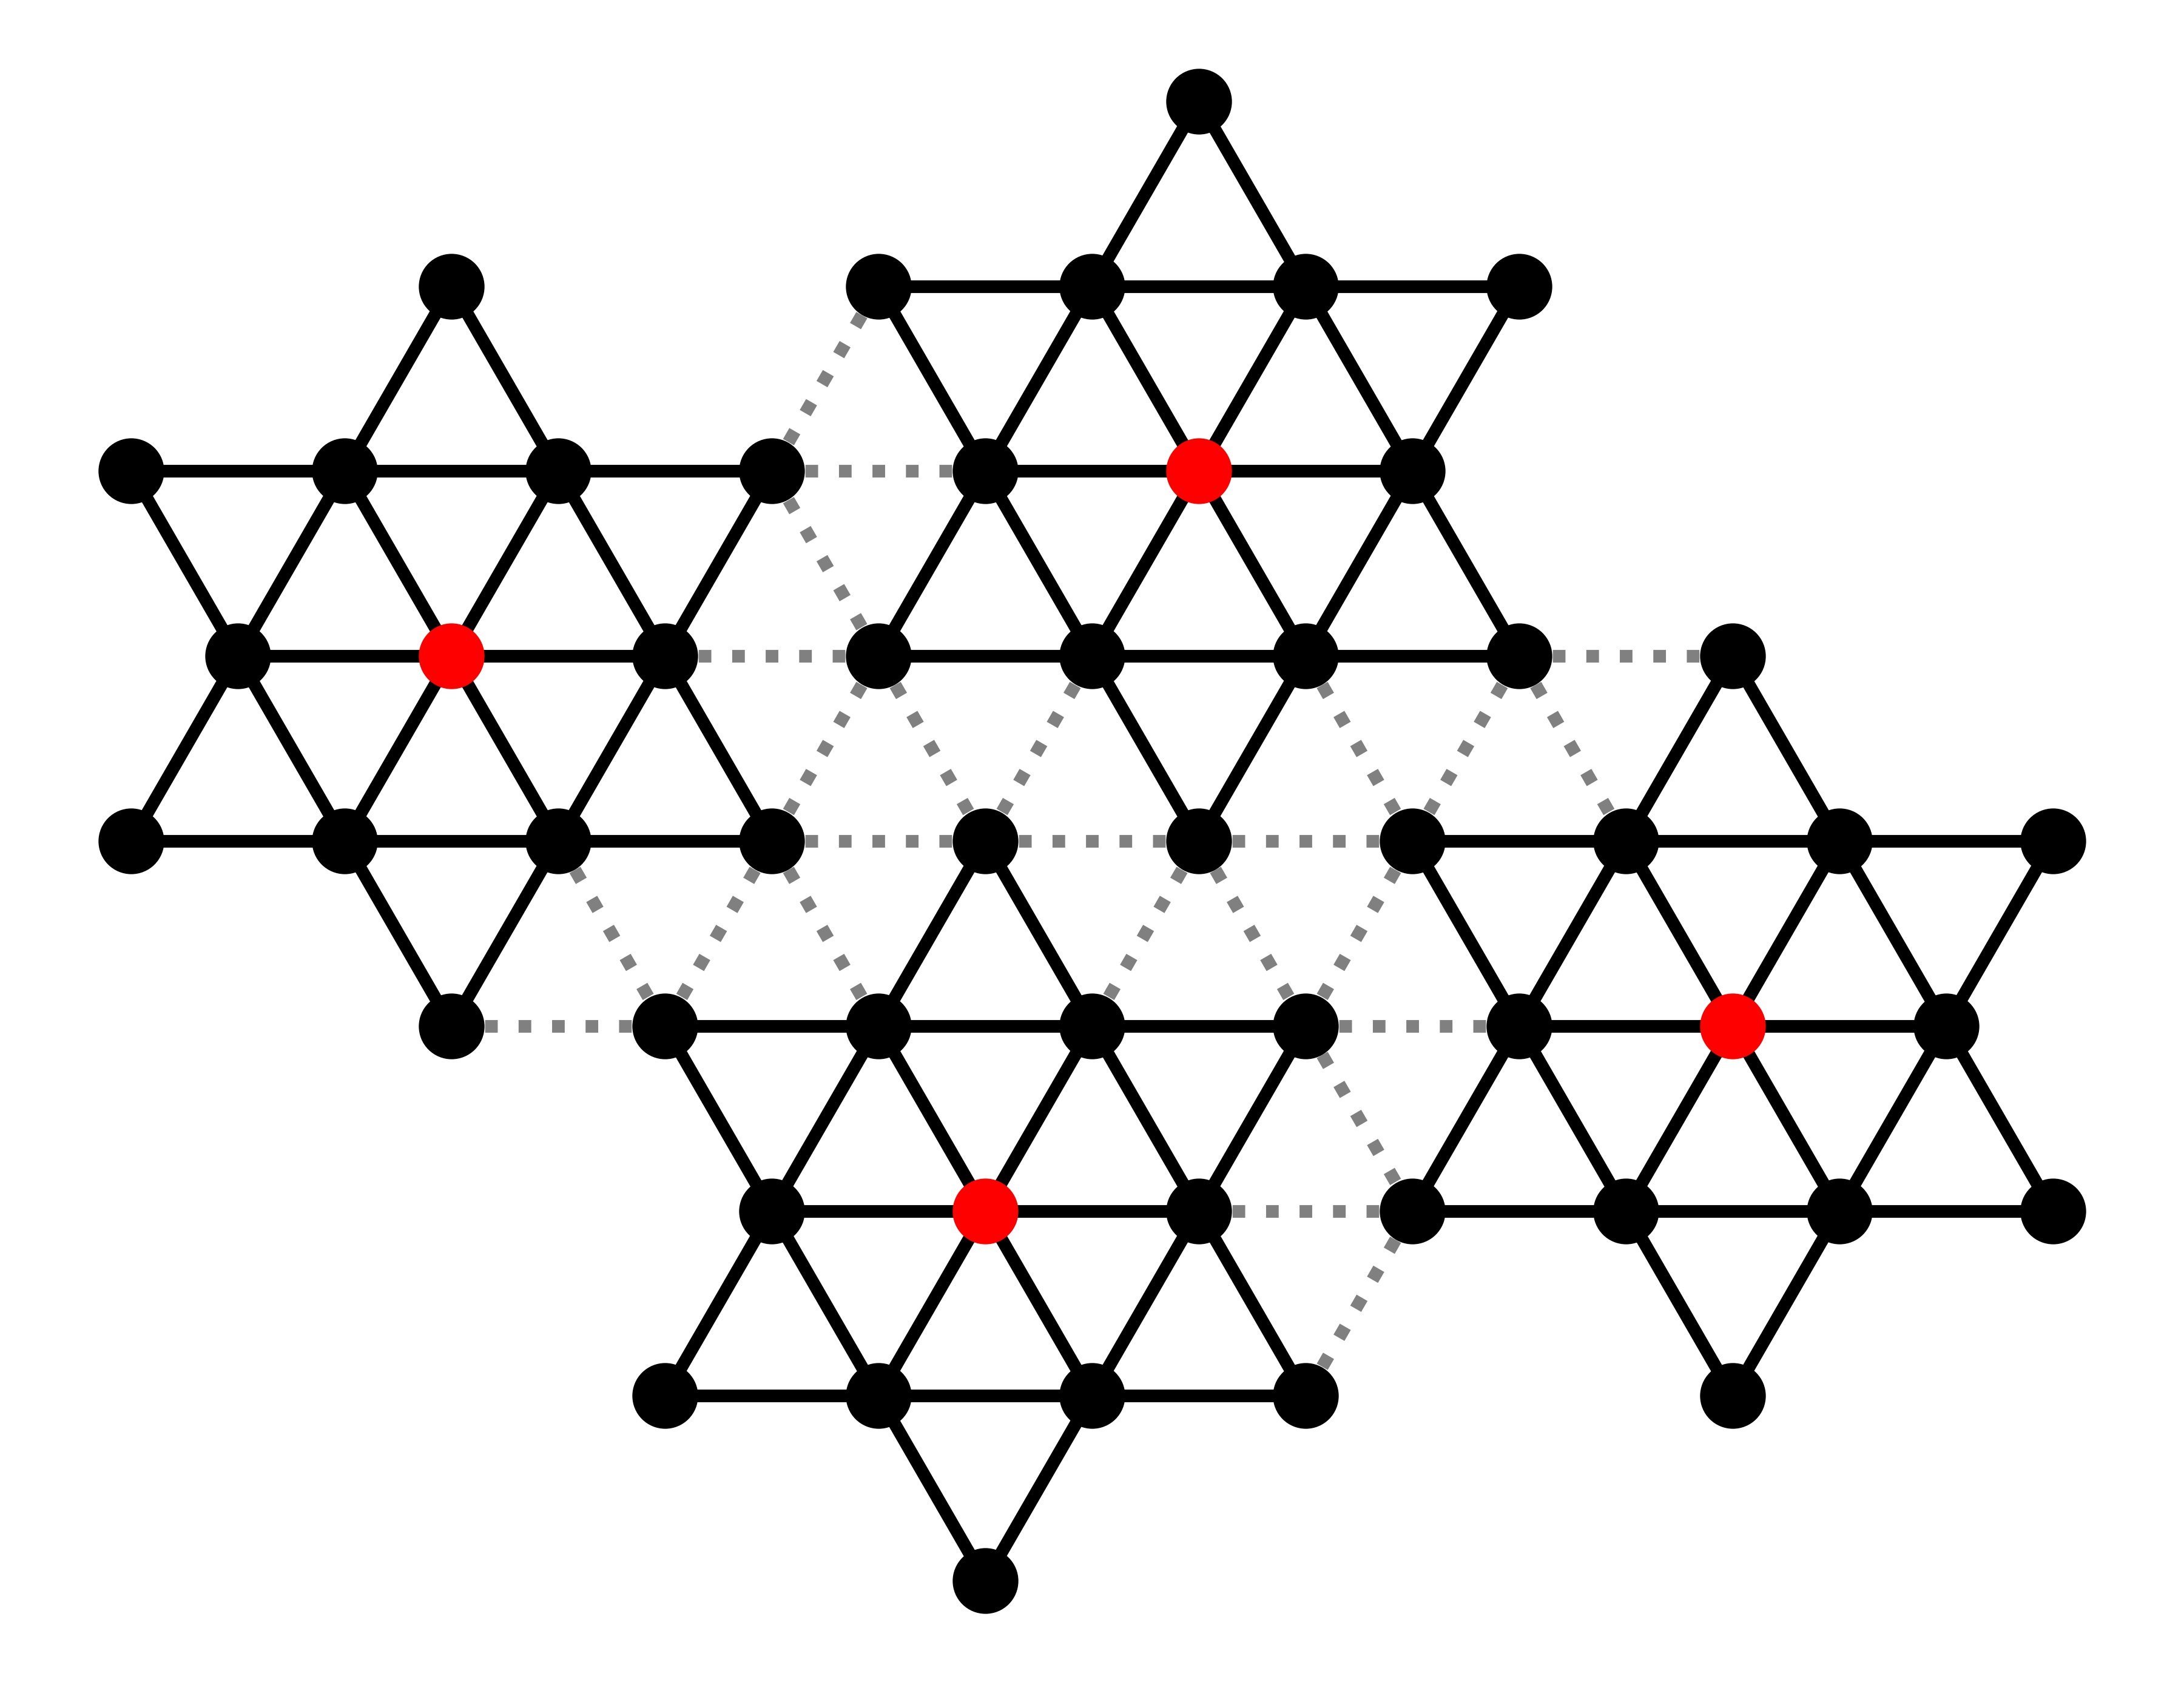
\includegraphics[scale=0.28]{fig/cpt-cluster.jpg}
  \caption{\label{cpt-cluster}Tiling of the triangular lattice with $13$-site clusters. The nearest-neighbor hoppings within a cluster are represented by solid lines, and intercluster hoppings by dashed lines. Here, each site represents a David star in $1$T-TaS$_{2}$, and the red sites are the David stars where the K$^{+}$ cations are located in the theoretical calculations.}
\end{figure}
In the main text, the computational technique for our calculation of the single-particle spectral weight $A_{i}(\omega)$ on site $i$ is based on the cluster perturbation theory (CPT), which has been successfully applied to many strongly correlated systems \cite{PhysRevLett.84.522,PhysRevLett.85.2585,PhysRevLett.92.126401,PhysRevLett.107.010401,PhysRevB.84.064520,PhysRevB.90.245102,PhysRevB.98.134410}. As shown in Fig.~\ref{cpt-cluster}, in the CPT calculations, we divide the original lattice into identical $13$-site clusters which constitute a superlattice. Then, the lattice Hamiltonian is written as
\begin{align}
H=H^{\prime}+V,
\end{align}
where $H^{\prime}$ is the cluster Hamiltonian, obtained by severing the hopping terms between different clusters, and $V$ contains the intercluster hoppings. The CPT method is based on a strong-coupling perturbation expansion of the one-body operators $V$ linking the individual clusters\cite{PhysRevLett.84.522}. At the lowest order of this expansion, the Green's function $\bm{G}$ of the original lattice can be expressed (in matrix form) as
\begin{align}
\bm{G}(\tilde{\bm{k}},\omega)=\bm{G}^{\prime}(\omega)[1-\bm{V}(\tilde{\bm{k}})\bm{G}^{\prime}(\omega)]^{-1},
\end{align}
where $\bm{G}^{\prime}$ is the cluster Green's function, and $\tilde{\bm{k}}$ is the wavevector in the Brillouin zone (BZ) of the superlattice. $\bm{G}^{\prime}$ is independent of $\tilde{\bm{k}}$, while $\bm{V}$ is frequency independent. The cluster Green's function $\bm{G}^{\prime}$ is calculated by the exact diagonalization method with the Lanczos algorithm, and it has the following expression,
\begin{align}
G^{\prime}_{\mu\nu}(\omega)&=\langle0|c_{\mu}\frac{1}{\omega-H+E_{0}+i\eta}c^{\dag}_{\nu}|0\rangle \nonumber \\
&+\langle0|c^{\dag}_{\nu}\frac{1}{\omega+H-E_{0}+i\eta}c_{\mu}|0\rangle,
\end{align}
where $E_{0}$ is the energy of the ground state $|0\rangle$, and $\eta$ is a small real number introduced in the calculation to shift the poles of the Green's function away from the real axis. Here, $\mu$ and $\nu$ denote both the site and spin degrees of freedom in a cluster.
The spectral function of the local single-particle excitation is given by
\begin{align}
A_{\mu\mu}(\omega)=-\frac{1}{\pi}\sum_{\tilde{\bm{k}}}G_{\mu\mu}(\tilde{\bm{k}},\omega).
\end{align}

\bibliography{1T-TaS2-supmat}

\end{document}
